
%(BEGIN_QUESTION)
% Copyright 2006, Tony R. Kuphaldt, released under the Creative Commons Attribution License (v 1.0)
% This means you may do almost anything with this work of mine, so long as you give me proper credit

In this process, water is separated from an oil stream by gravity.  The oil floats to the top of the vessel where it exits, while the water settles to the bottom and is drained off periodically by opening a hand valve.  A hydrostatic level transmitter detects the height of the oil/water interface and lets the human operator know when to open up the water drain valve:

$$\includegraphics[width=15.5cm]{i00309x01.eps}$$

Calculate values for the following calibration table, such that the transmitter will register the height of the oil/water interface from 0 to 6 feet off the bottom of the vessel.  Note that the oil/air interface is held at a constant 9 feet of level by the position of the overflow tube.  Assume a vapor pressure inside the vessel of 2.53 PSI and a transmitter calibration tolerance of +/- 0.25\%:

% No blank lines allowed between lines of an \halign structure!
% I use comments (%) instead, so that TeX doesn't choke.

$$\vbox{\offinterlineskip
\halign{\strut
\vrule \quad\hfil # \ \hfil & 
\vrule \quad\hfil # \ \hfil & 
\vrule \quad\hfil # \ \hfil & 
\vrule \quad\hfil # \ \hfil & 
\vrule \quad\hfil # \ \hfil & 
\vrule \quad\hfil # \ \hfil \vrule \cr
\noalign{\hrule}
%
% First row
Interface & Percent of & $\Delta$ pressure & Output signal & Output signal & Output signal \cr
%
% Another row
level (ft) & span (\%) & sensed ("W.C) & ideal (PSI) & min. (PSI) & max. (PSI) \cr
%
\noalign{\hrule}
%
% Another row
  & 0 &  &  &  &  \cr
%
\noalign{\hrule}
%
% Another row
  & 10 &  &  &  &  \cr
%
\noalign{\hrule}
%
% Another row
  & 25 &  &  &  &  \cr
%
\noalign{\hrule}
%
% Another row
  & 50 &  &  &  &  \cr
%
\noalign{\hrule}
%
% Another row
  & 75 &  &  &  &  \cr
%
\noalign{\hrule}
%
% Another row
  & 90 &  &  &  &  \cr
%
\noalign{\hrule}
%
% Another row
  & 100 &  &  &  &  \cr
%
\noalign{\hrule}
} % End of \halign 
}$$ % End of \vbox

\vskip 20pt \vbox{\hrule \hbox{\strut \vrule{} {\bf Suggestions for Socratic discussion} \vrule} \hrule}

\begin{itemize}
\item{} Demonstrate how to {\it estimate} numerical answers for this problem without using a calculator.
\item{} How will this level transmitter respond if the gas pressure inside this vessel were to increase?
\item{} How will this level transmitter respond if the gas pressure inside this vessel were to decrease?
\item{} How will this level transmitter respond if the overflow pipe were to be blocked off, so no light liquid could exit the vessel?
\item{} How will this level transmitter respond if some liquid enters the otherwise ``dry'' compensating leg?
\end{itemize}

\underbar{file i00309}
%(END_QUESTION)





%(BEGIN_ANSWER)

Here are the two ``thought experiment'' scenarios pictured to arrive at the LRV and URV pressure values:

$$\includegraphics[width=15.5cm]{i00309x02.eps}$$

% No blank lines allowed between lines of an \halign structure!
% I use comments (%) instead, so that TeX doesn't choke.

$$\vbox{\offinterlineskip
\halign{\strut
\vrule \quad\hfil # \ \hfil & 
\vrule \quad\hfil # \ \hfil & 
\vrule \quad\hfil # \ \hfil & 
\vrule \quad\hfil # \ \hfil & 
\vrule \quad\hfil # \ \hfil & 
\vrule \quad\hfil # \ \hfil \vrule \cr
\noalign{\hrule}
%
% First row
Interface & Percent of & $\Delta$ pressure & Output signal & Output signal & Output signal \cr
%
% Another row
level (ft) & span (\%) & sensed ("W.C) & ideal (PSI) & min. (PSI) & max. (PSI) \cr
%
\noalign{\hrule}
%
% Another row
0 & 0 & 86.4 & 3 & 2.97 & 3.03 \cr
%
\noalign{\hrule}
%
% Another row
0.6 & 10 & 87.84 & 4.2 & 4.17 & 4.23 \cr
%
\noalign{\hrule}
%
% Another row
1.5 & 25 & 90.0 & 6 & 5.97 & 6.03 \cr
%
\noalign{\hrule}
%
% Another row
3 & 50 & 93.6 & 9 & 8.97 & 9.03 \cr
%
\noalign{\hrule}
%
% Another row
4.5 & 75 & 97.2 & 12 & 11.97 & 12.03 \cr
%
\noalign{\hrule}
%
% Another row
5.4 & 90 & 99.36 & 13.8 & 13.77 & 13.83 \cr
%
\noalign{\hrule}
%
% Another row
6  & 100 & 100.8 & 15 & 14.97 & 15.03 \cr
%
\noalign{\hrule}
} % End of \halign 
}$$ % End of \vbox

\vskip 10pt


%(END_ANSWER)





%(BEGIN_NOTES)

The vapor pressure inside the vessel is extraneous information, included for the purpose of challenging students to identify whether or not information is relevant to solving a particular problem.

%INDEX% Measurement, interface level: calibration table

%(END_NOTES)


